\documentclass{jlreq}
\usepackage{float}
\usepackage{graphicx}

\title{人工生命と進化型計算}
\author{学籍番号: 02230471 氏名: 佐藤雅文}
\date{提出日: 2026年2月4日}

\begin{document}
\maketitle

\section {パーコレーション}
% イントロダクション
全体として、正方格子/三角格子のボンド/サイトパーコレーションのシミュレーション、また臨界確率に関する考察を行った。
\par
実装したシミュレーションコードと、それによって得られた結果(csvファイル)も、percolationフォルダの中に格納している。
\par
シミュレーションでは、パーコレーションモデルをUnion-Find法をベースに実装した。
Union-Find法とは、グループを木構造で管理する方法であり、
グループ同士を結合するUnionと要素が属するグループの根要素がどれかを探すFindの2つの操作からなる。
Findする際に、辿って通った要素全てを直接根要素に付け替えながら根要素を探すので、
木構造が浅くなり、親要素を辿る操作が非常に速いことに特徴がある。
\par
また、パーコレーションモデルでは、その最上辺の格子点にひとつでも水が流れていて、
かつ最下辺の格子点にひとつでも水が流れているかどうかを浸透の判定基準とし、
開いている点または辺を繋いでいく作業をUnion-Find法のUnionの操作に対応させ、
最上辺と最下辺がつながっているかどうかを判定する。
\par
なお、コード上では簡単のため、最上辺と最下辺をそれぞれ全て仮想の点VirtualTopとVirtualBottomにUnionし、
VirtualTopとVirtualBottomがUnionされているかを浸透の基準としている。
\par
シミュレーションコードはJavaで実装した。
その際のクラス図は以下の図のようである。

\begin{figure}
    \centering
    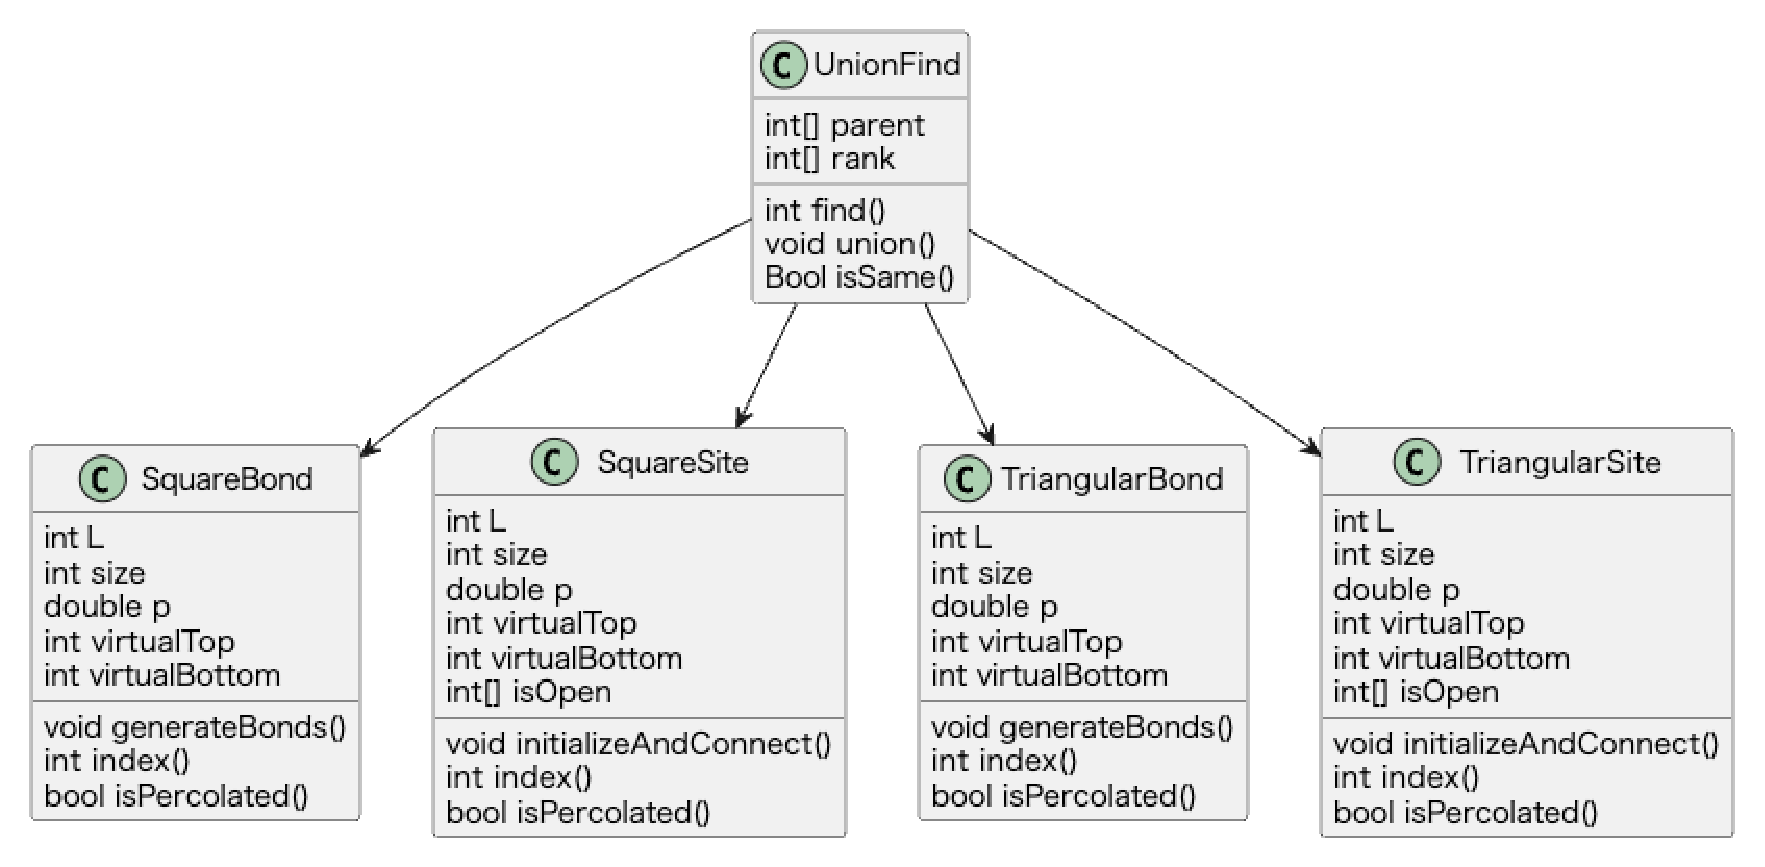
\includegraphics[width=0.8\linewidth]{percolationClassUML.eps}
    \caption{パーコレーションモデルクラス図}
\end{figure}

\subsection{正方格子ボンドパーコレーション}
% シミュレーション結果
シミュレーションは、以下の条件で行った。\par
\begin{itemize}
    \item 1辺の長さL: 401
    \item 試行回数: 2000
\end{itemize}
シミュレーションを行った結果、占有確率に対する浸透確率の値は以下のグラフのように遷移した。
% \begin{figure}
%     \centering
%     \includegraphics[options]{name}
%     \caption{正方格子ボンドパーコレーションの浸透確率遷移}
% \end{figure}

% 考察
グラフから、占有確率$p=0.5$近くで浸透確率が0より大きくなり始めていることが読み取れる。
厳密には、初めて浸透確率が0より大きくなったのは$p=$ !!!! のときだが、
その後も0に戻ることがなくなるような確率は$p=$ !!!! であった。(参照→./percolation/SquareBond.csv)
\par
これは、正方格子ボンドパーコレーションの臨界確率として既によく知られていて、厳密に求められている値$p=0.5$とよく一致していている。
\par
今回は、$p=$ !!! から浸透確率が緩やかなカーブを描いて1に近づいていった。
しかし、理論上ではサイズLが無限大になると、$p=0.5$で浸透確率が0から1に不連続に変化することが知られていて、
サイズLが小さければ小さいほどグラフの遷移が緩やかになっていく。
!!!!
これを確かめたのが以下の図
% \begin{figure}
%     \centering
%     \includegraphics[options]{name}
%     \caption{グラフの遷移の検証}
% \end{figure}
諸条件は以下の通り


\subsection{正方格子サイトパーコレーション}
%シミュレーション結果
シミュレーションは、以下の条件で行った。\par
\begin{itemize}
    \item 1辺の長さL: 501
    \item 試行回数: 5000
\end{itemize}
シミュレーションを行った結果、占有確率に対する浸透確率の値は以下のグラフのように遷移した。
% \begin{figure}
%     \centering
%     \includegraphics[options]{name}
%     \caption{正方格子サイトパーコレーションの浸透確率遷移}
% \end{figure}

% 考察
グラフから、占有確率$p=0.59$近くで浸透確率が0より大きくなり始めていることが読み取れる。
これも厳密には初めて浸透確率が0より大きくなったのは、$p=$ !!! のときだが、
その後も0に戻ることがなくなるような確率は$p= $ !!!! であった。(参照→./percolation/SquareSite.csv)
\par
これは、正方格子サイトパーコレーションの臨界確率としてすでに知られている値$p=0.5927$とよく一致している。
これは、厳密に解析的に求められた解ではないが、数値的に求められている。
\par
正方格子において、ボンドパーコレーションよりサイトパーコレーションのほうが臨界確率が高いのは、
サイトが閉じると、そこにつながるすべての結合が遮断されるため、ボンドパーコレーションよりも厳しい条件になるからであると考えられる。


\subsection{三角格子ボンドパーコレーション}
% シミュレーション結果
シミュレーションは、以下の条件で行った。\par
% \begin{figure}
%     \centering
%     \includegraphics[options]{name}
%     \caption{三角格子ボンドパーコレーションの浸透確率遷移}
% \end{figure}

% 考察
グラフから、占有確率$p=$近くで浸透確率が0より大きくなり始めていることが読み取れる。
これも厳密には初めて浸透確率が0より大きくなったのは、$p= $ !!! のときだが、
その後も0に戻ることがなくなるような確率は$p=$ !!! であった。(参照→./percolation/TriangularBond.csv)
\par
これは、三角格子ボンドパーコレーションの臨界確率としてすでによく知られていて、厳密に求められている$p=2sin(\frac{\pi}{18})\neq0.3473$値と一致している。
\par
正方格子のボンドパーコレーションよりも臨界確率が低いのは、
1つの格子点に対してつながっている辺の数(配位数)が6辺となり迂回路がたくさんあるため、
浸透しやすくなるためであると考えられる。
\begin{table}
    \centering
    \begin{tabular}{|c|c|c|}
        \hline
        & 配位数 & 臨界確率 \\
        \hline
        正方格子ボンドパーコレーション & 4 & 0.5 \\
        \hline
        三角格子ボンドパーコレーション & 6 & 0.34729\dots \\
        \hline
    \end{tabular}
    \caption{正方格子と三角格子の違いと臨界確率}
\end{table}


\subsection{三角格子サイトパーコレーション}
% シミュレーション結果
シミュレーションは以下の条件で行った。

% \begin{figure}
%     \centering
%     \includegraphics[options]{name}
%     \caption{三角格子サイトパーコレーションの浸透確率遷移}
% \end{figure}

% 考察
グラフから、占有確率$p=$近くで浸透確率が0より大きくなり始めていることが読み取れる。
これも厳密には初めて浸透確率が0より大きくなったのは、$p= $ !!! のときだが、
その後も0に戻ることがなくなるような確率は$p=$ !!! であった。(参照→./percolation/TriangularSite.csv)
\par
ここまで触れてきたように、臨界確率が正方格子のサイトパーコレーションに比べ低く、
三角格子のボンドパーコレーションに比べて高い。

\subsubsection*{まとめ}
正方格子/三角格子では正方格子のほうが臨界確率が低く、
ボンド/サイトではサイトパーコレーションのほうが臨界確率が低い。
これらをまとめると以下の表のようになる。

\begin{table}
    \centering
    \begin{tabular}{|c|c|c|c||}
        \hline
        正方格子/三角格子 & ボンド/サイト & 配位数 & 臨界確率 \\
        \hline
        正方格子 & ボンド & 4 & 0.5 \\
        \hline
        正方格子 & サイト & 4 & 0.5927 \\
        \hline
        三角格子 & ボンド & 6 & 0.34729\dots \\
        \hline
        三角格子 & サイト & 6 & 0.5 \\
        \hline
    \end{tabular}
    \caption{各パーコレーションモデルの比較}
\end{table}

また、有限サイズ効果により、シミュレーションの結果上では、浸透確率の臨界確率での立ち上がりがゆっくりとしているが、
無限大のサイズでは不連続に0から1に飛ぶことが知られている。


\section{遺伝的アルゴリズム}
% イントロダクション
この課題では、GAによりTSPの解の探索を行い、各種パラメータに関する考察を行った。
\par
アルゴリズムの実装はJavaで行った。
実装したコードは./geneticAlgorithmフォルダの中に格納している。
\par
GAのアルゴリズムの実装にあたっては、以下のようなクラス構造とした。
\begin{figure}
    \centering
    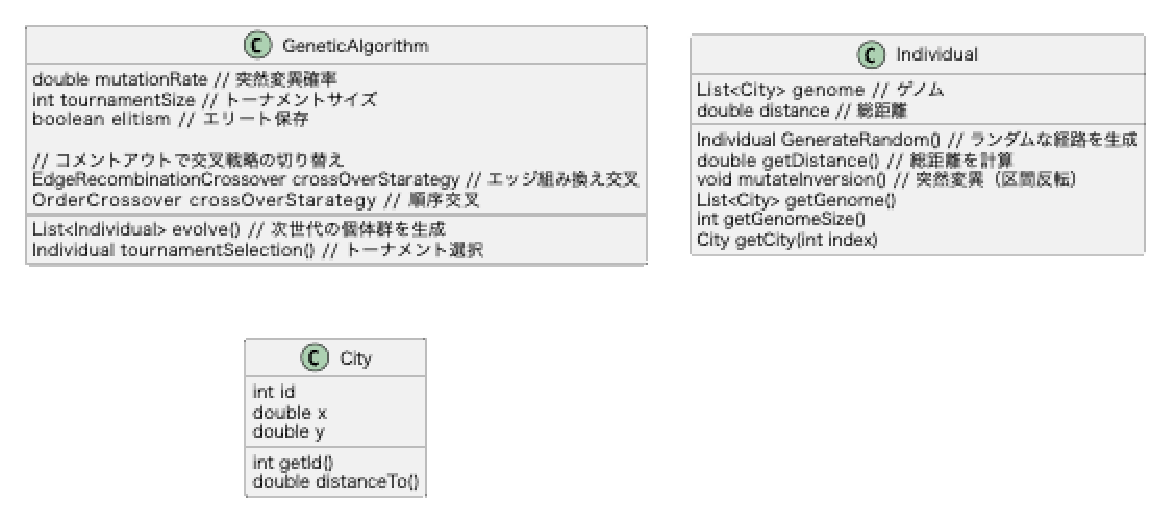
\includegraphics[width=0.8\linewidth]{./geneticAlgorithmClassUML.eps}
    \caption{GAによるTSPの最適解探索アルゴリズムクラス図}
\end{figure}

\subsection{各種パラメータ値による比較}
各種パラメータ値によるGAの性能差の比較のため、以下の各パラメータについてその値を変更し、
得られる解がどのように変化するかを検証した。
\begin{itemize}
    \item 個体数
    \item 突然変異確率
    \item トーナメントサイズ
    \item エリート保存(の有無)
\end{itemize}
\par
なお、検証の際には、収束に十分な世代数として全ての場合で5000世代の進化を繰り返して得られた値を結果として採用した。
また、パラメータの組み合わせの評価には、50回の試行で得られた平均値と標準偏差を指標とする。

% 個体数による比較
\subsubsection*{個体数}
個体数を変化させたときの各種パラメータの値と、そのときのスコアは以下のように変化した。

\begin{table}
    \centering
    \begin{tabular}{|c|c|c|c|c|c|c|}
        \hline
        & 個体数 & 突然変異確率 & トーナメントサイズ & エリート保存 & スコア平均値 & スコア標準偏差 \\
        \hline
        試験1 & 10 & 0.05 & 5 & true & 111.11\\
        試験1 & 100 & 0.05 & 5 & true & 111.11\\
        試験1 & 1000 & 0.05 & 5 & true & 111.11\\
        
        試験1 & 10 & 0.05 & 10 & true & 111.11\\
        試験1 & 10 & 0.05 & 40 & true & 111.11\\
        試験1 & 100 & 0.05 & 10 & true & 111.11\\
        試験1 & 100 & 0.05 & 40 & true & 111.11\\
        試験1 & 1000 & 0.05 & 10 & true & 111.11\\
        試験1 & 1000 & 0.05 & 40 & true & 111.11\\
        試験1 & 10 & 0.05 & 5 & false & 111.11\\
        試験1 & 10 & 0.05 & 10 & false & 111.11\\
        試験1 & 10 & 0.05 & 40 & false & 111.11\\
        試験1 & 100 & 0.05 & 5 & false & 111.11\\
        試験1 & 100 & 0.05 & 10 & false & 111.11\\
        試験1 & 100 & 0.05 & 40 & false & 111.11\\
        試験1 & 1000 & 0.05 & 5 & false & 111.11\\
        試験1 & 1000 & 0.05 & 10 & false & 111.11\\
        試験1 & 1000 & 0.05 & 40 & false & 111.11\\
        
        \hline
    \end{tabular}
    \caption{個体数による比較のための実験}
\end{table}


% 突然変異確率による比較
\subsubsection*{突然変異確率}
突然変異確率を変化させたときの各種パラメータの値と、そのときのスコアは以下のように変化した。

\begin{table}
    \centering
    \begin{tabular}{|c|c|c|c|c|c|c|}
        \hline
        & 個体数 & 突然変異確率 & トーナメントサイズ & エリート保存 & スコア平均値 & スコア標準偏差 \\
        \hline
        試験1 & 100 & 0.05 & 5 & true & 111.11\\
        試験1 & 100 & 0.05 & 10 & true & 111.11\\
        試験1 & 100 & 0.05 & 40 & true & 111.11\\
        \hline
    \end{tabular}
    \caption{突然変異確率による比較のための実験}
\end{table}


% トーナメントサイズによる比較
\subsubsection*{トーナメントサイズ}
トーナメントaiを変化させたときの各種パラメータの値と、そのときのスコアは以下のように変化した。

\begin{table}
    \centering
    \begin{tabular}{|c|c|c|c|c|c|c|}
        \hline
        & 個体数 & 突然変異確率 & トーナメントサイズ & エリート保存 & スコア平均値 & スコア標準偏差 \\
        \hline
        試験1 & 10 & 0.05 & 5 & true & 111.11\\
        試験1 & 100 & 0.05 & 5 & true & 111.11\\
        試験1 & 1000 & 0.05 & 5 & true & 111.11\\
        
        試験1 & 10 & 0.05 & 10 & true & 111.11\\
        試験1 & 10 & 0.05 & 40 & true & 111.11\\
        試験1 & 100 & 0.05 & 10 & true & 111.11\\
        試験1 & 100 & 0.05 & 40 & true & 111.11\\
        試験1 & 1000 & 0.05 & 10 & true & 111.11\\
        試験1 & 1000 & 0.05 & 40 & true & 111.11\\
        試験1 & 10 & 0.05 & 5 & false & 111.11\\
        試験1 & 10 & 0.05 & 10 & false & 111.11\\
        試験1 & 10 & 0.05 & 40 & false & 111.11\\
        試験1 & 100 & 0.05 & 5 & false & 111.11\\
        試験1 & 100 & 0.05 & 10 & false & 111.11\\
        試験1 & 100 & 0.05 & 40 & false & 111.11\\
        試験1 & 1000 & 0.05 & 5 & false & 111.11\\
        試験1 & 1000 & 0.05 & 10 & false & 111.11\\
        試験1 & 1000 & 0.05 & 40 & false & 111.11\\
        
        \hline
    \end{tabular}
    \caption{個体数による比較のための実験}
\end{table}




\end{document}